\chapter{背景理論付きSAT}\label{chap:smt}

%%%%%%%%%%%%%%%%%%%%%%%%%%%%%%%%%%%%%%%%%%%%%%%%
%
% SMTとは
%
%%%%%%%%%%%%%%%%%%%%%%%%%%%%%%%%%%%%%%%%%%%%%%%%
\section{SMTとSMTソルバー}
SMT(背景理論付きSAT)は,命題論理よりも高い表現力を持つ論理体系で記述された背景理論をSAT技術で効果的に扱うことを目的とした技術である.
SATが命題論理を扱うのに対して,SMTでは述語論理を扱う\cite{JSAI:IwanumaN10}.

%%%%%%%%%%%%%%%%%%%%%%%%%%%%%%%%%%%%%%%%%%%%%%%%
%
% SNTソルバーとは
%
%%%%%%%%%%%%%%%%%%%%%%%%%%%%%%%%%%%%%%%%%%%%%%%%
% \section{SMTソルバーとは}
SMTソルバーは,プログラム検証,スケジューリング,プランニングなどの場面に使用される.


% \subsection{smt-lib2とは}
今回SMTソルバーを扱う際に使用する記述方法はsmt-lib2である.
SMT-LIBはSMTの研究開発の促進を目的とした国際的な取り組みであり,
その目的としては,
SMTシステムで使用される背景理論の標準的で厳密な記述の提供や
SMTソルバーのための共通の入出力言語を開発し促進することなどが挙げられる.


% distinct制約とは
本研究で扱う$distinct$制約とは,$(distinct x_1 ... x_n)$で表され,その要素$x_i$が互いに異なることを表す制約である.
今回使用したSMTソルバーの$z3ソルバー$においてこの制約は以下のことを意味する.
\begin{eqnarray*}
    \bigwedge_{1 \leq i < j \leq n} x_i \neq x_j
\end{eqnarray*}


% \subsection{背景理論}
SMTで扱われる背景理論には等号や算術,配列やリスト,ビットベクターなどが挙げられる.

% \subsection{既存のSMTソルバー}
既存のSMTソルバーとしては,OpenSMT,YICES,UCLID,CVC3,Z3などが挙げられる.
今回使用したソルバーは$z3ソルバー$である.Microsoft社によって開発されたもので,プログラム解析やテスト,検証などを目的としている\cite{Umemura10:jssst}.


\section{プログラム例}


%%%%%%%%%%%%%%%%%%%%%%%%%%%%%%%%%%%%%%%%%%%%%%%%
%
% プログラム例
%
%%%%%%%%%%%%%%%%%%%%%%%%%%%%%%%%%%%%%%%%%%%%%%%%
% \section{プログラム例}
\begin{figure}[tb]
  \centering
  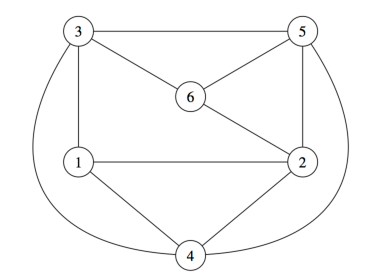
\includegraphics[width=0.6\linewidth]{fig/graph3.pdf}
  \caption{グラフ}
  \label{fig:graph}
\end{figure}
smt-lib2形式でのプログラムの例をグラフ彩色問題を用いて説明する.
使用するSMTソルバーは$z3ソルバー(ver.4.8.9)$とする.

グラフ彩色問題とは,辺で結ばれたノードが同じ色にならないように,各ノー
ドを塗り分ける問題である.
例として,図~\ref{fig:graph}のグラフを赤(1),青(2),緑
(3)の3色で塗り分ける問題を考える.
この問題を表すプログラムをコード~\ref{code:color.smt2}に示す.

2から7行目は整数変数の宣言をしている.ここではx\_iのiがノード番号を表している.
8から13行目はx\_iは3色に塗り分けられるため,1以上3以下であるという制約を追加している.
14から23行目は辺で結ばれたノードの色が同じにならないことを等号を使って表している.
24行目はそのプログラムに解が存在するかどうかをチェックし出力することを表し,
25行目は求められた解を出力する.
26行目はプログラムの終わりを表す.

コード\ref{code:color.smt2}の$z3ソルバー$での実行例をコード\ref{code:color.log}に示す.
この出力から,ノード2と3は赤,ノード1と5は青,ノード4と6は緑に塗り分けられることがわかる.

\lstinputlisting[float=htbp,caption={%
グラフ彩色問題のプログラム (\code{color.smt2})},%
captionpos=b,frame=single,label=code:color.smt2,%
numbers=left,%
breaklines=true,%
columns=fullflexible,keepspaces=true,%
basicstyle=\ttfamily\scriptsize]{code/color.smt2}
%%%%%%%%%%%%%%%%%%%%%%%%%%%%%%%%%
\lstinputlisting[float=htbp,caption={%
\code{color.smt2}に対する$z3ソルバー$の実行例},%
captionpos=b,frame=single,label=code:color.log,%
numbers=none,%
breaklines=true,%
columns=fullflexible,keepspaces=true,%
basicstyle=\ttfamily\scriptsize]{code/color.log}
%%%%%%%%%%%%%%%%%%%%%%%%%%%%%%%%%



%%%%%%%%%%%%%%%%%%%%%%%%%%%%%%%%%%%%%%%%%%%%%%%%
\section{$distinct$制約}
%%%%%%%%%%%%%%%%%%%%%%%%%%%%%%%%%%%%%%%%%%%%%%%%

\begin{itemize}
\item $distinct$制約とは...
\item $distinct$制約の実装方法.($\neq$分解, PB符号化)
  
\end{itemize}



%%% Local Variables:
%%% mode: japanese-latex
%%% TeX-master: "paper"
%%% End:
